\documentclass[10pt,aspectratio=169]{beamer}

\usepackage[T1]{fontenc}
\usepackage[utf8]{inputenc}
\usepackage[english]{babel}

\usepackage[protrusion=true,expansion=false]{microtype}
\usepackage{amsmath,amssymb,bm}
\usepackage{array,booktabs,tabularx}
\usepackage{graphicx}
\usepackage{xcolor}
\usepackage{tikz}
\usepackage{pgfplots}
\usepackage{appendixnumberbeamer}

\usetikzlibrary{arrows.meta,calc,fit,positioning,shapes.geometric}
\pgfplotsset{compat=1.18}

\usetheme{Madrid}
\useinnertheme{rectangles}
\usecolortheme{default}

\definecolor{ink}{HTML}{1F2529}
\definecolor{muted}{HTML}{6B7378}
\definecolor{accent}{HTML}{0B5FA5}
\definecolor{accentlight}{HTML}{EAF2FB}
\definecolor{signal}{HTML}{C46A1A}
\definecolor{signalsoft}{HTML}{FCE9D9}
\definecolor{linegray}{HTML}{D9E2EC}
\definecolor{softgray}{HTML}{EEF2F7}

\setbeamercolor{background canvas}{bg=white}
\setbeamercolor{normal text}{fg=ink,bg=white}
\setbeamercolor{title}{fg=white}
\setbeamercolor{subtitle}{fg=white}
\setbeamercolor{titlelike}{fg=white,bg=accent}
\setbeamercolor{frametitle}{fg=white,bg=accent}
\setbeamercolor{framesubtitle}{fg=accent,bg=white}
\setbeamercolor{structure}{fg=accent}
\setbeamercolor{block title}{fg=white,bg=accent}
\setbeamercolor{block body}{fg=ink,bg=accentlight}
\setbeamercolor{alerted text}{fg=signal}

\setbeamerfont{title}{size=\Large,series=\bfseries}
\setbeamerfont{subtitle}{size=\normalsize}
\setbeamerfont{frametitle}{size=\large,series=\bfseries}
\setbeamerfont{framesubtitle}{size=\small,series=\mdseries}

\setbeamertemplate{navigation symbols}{}
\setbeamertemplate{items}[triangle]
\setbeamertemplate{blocks}[rounded][shadow=false]
\setbeamersize{text margin left=0.6cm,text margin right=0.6cm}
\setlength{\parskip}{0.2em}
\setlength{\tabcolsep}{4pt}
\renewcommand{\arraystretch}{1.12}

\setbeamertemplate{footline}[frame number]

\newcolumntype{L}[1]{>{\raggedright\arraybackslash}p{#1}}
\newcolumntype{C}[1]{>{\centering\arraybackslash}p{#1}}
\newcolumntype{R}[1]{>{\raggedleft\arraybackslash}p{#1}}

\newcommand{\papersource}[1]{{\tiny\color{muted}Source: #1}}
\newcommand{\callout}[1]{%
  \begin{beamercolorbox}[wd=\linewidth,rounded=true,sep=0.18cm,shadow=false]{block body}
  \raggedright #1
  \end{beamercolorbox}
}
\newcommand{\metricdown}{\ensuremath{\downarrow}}
\newcommand{\metricup}{\ensuremath{\uparrow}}

\newcommand{\papercrop}[3][]{%
  \includegraphics[#1,page=#2,trim=#3,clip]{../REPA/Representation_Alignment_.pdf}%
}

\newcommand{\FigOne}[1][]{\papercrop[#1]{1}{54bp 250bp 63bp 445bp}}
\newcommand{\FigTwo}[1][]{\papercrop[#1]{2}{50bp 598bp 63bp 50bp}}
\newcommand{\FigThree}[1][]{\papercrop[#1]{3}{50bp 598bp 63bp 47bp}}
\newcommand{\FigFour}[1][]{\papercrop[#1]{5}{43bp 625bp 59bp 48bp}}
\newcommand{\FigFive}[1][]{\papercrop[#1]{8}{38bp 625bp 59bp 55bp}}
\newcommand{\FigSix}[1][]{\papercrop[#1]{8}{66bp 165bp 60bp 345bp}}
\newcommand{\FigNine}[1][]{\papercrop[#1]{20}{190bp 515bp 200bp 110bp}}
\newcommand{\FigTen}[1][]{\papercrop[#1]{21}{95bp 260bp 144bp 270bp}}
\newcommand{\FigEleven}[1][]{\papercrop[#1]{26}{210bp 540bp 205bp 120bp}}
\newcommand{\AppQuant}[1][]{\papercrop[#1]{25}{32bp 99bp 36bp 41bp}}
\newcommand{\AppFiveTwelve}[1][]{\papercrop[#1]{30}{108bp 270bp 102bp 245bp}}
\newcommand{\AppTTwoI}[1][]{\papercrop[#1]{31}{72bp 170bp 88bp 275bp}}
\newcommand{\AppFeature}[1][]{\papercrop[#1]{32}{75bp 150bp 75bp 365bp}}
\newcommand{\AppQualTop}[1][]{\papercrop[#1]{27}{40bp 525bp 50bp 96bp}}
\newcommand{\AppQualBottom}[1][]{\papercrop[#1]{27}{40bp 270bp 50bp 370bp}}

\title[REPA]{Representation Alignment for Generation}
\subtitle{Training Diffusion Transformers Is Easier Than You Think}
\author[Yu et al.]{Sihyun Yu et al.}
\institute[Reading Group]{Reading Group Deck}
\date[ICLR 2025]{ICLR 2025}

\begin{document}

\begin{frame}
  \titlepage
  \vspace{-0.2cm}
  \begin{block}{Talk goal}
    Explain why diffusion transformers suffer from a representation bottleneck,
    how REPA turns that bottleneck into an explicit alignment objective, and why the payoff is
    both faster convergence and better final FID.
  \end{block}
\end{frame}

\begin{frame}[t]
  \framesubtitle{One-Slide Summary}
  \frametitle{Thesis: make representation learning explicit}
  \begin{columns}[T,totalwidth=\textwidth]
    \column{0.47\textwidth}
    \callout{\textbf{Core idea.} Instead of hoping a diffusion transformer will discover strong
    semantics only through denoising, REPA explicitly aligns an early hidden state with a clean
    representation from a pretrained encoder such as DINOv2.}
    \vspace{0.18cm}
    \begin{itemize}
      \item Hidden states become semantically stronger earlier in training.
      \item Later layers can spend more capacity on high-frequency refinement.
      \item The same model family gets both faster convergence and better sample quality.
    \end{itemize}
    \vspace{0.1cm}
    \begin{beamercolorbox}[wd=\linewidth,rounded=true,sep=0.18cm]{block body}
      \textbf{Headline result.} For SiT-XL/2, REPA matches or exceeds the vanilla 7M-step regime
      in a small fraction of the training budget.
    \end{beamercolorbox}
  \column{0.51\textwidth}
    \FigOne[width=\linewidth]
  \end{columns}
\end{frame}

\begin{frame}[t]
  \framesubtitle{Problem}
  \frametitle{Why representation quality is the bottleneck}
  \begin{columns}[T,totalwidth=\textwidth]
    \column{0.53\textwidth}
    \begin{itemize}
      \item A denoising model must recover both \textit{semantics} and \textit{fine detail} from noisy latents.
      \item Pure reconstruction pressure is weak supervision for learning noise-invariant, discriminative features.
      \item So a large transformer wastes training budget on discovering semantics that modern SSL encoders already capture well.
    \end{itemize}
    \vspace{0.18cm}
    \callout{\textbf{Paper hypothesis.} The hard part of training DiT/SiT is not only solving the
    denoising objective; it is learning an internal representation that is good enough to support generation.}
    \vspace{0.18cm}
    {\small
    Denoising gives an implicit encoder \(f_\theta(z_t)=h_t\), but nothing guarantees that \(h_t\)
    will align with the semantic structure learned by strong visual encoders.}
  \column{0.43\textwidth}
    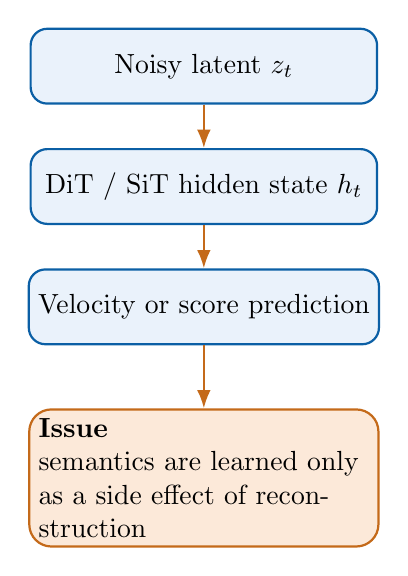
\begin{tikzpicture}[>=Latex,thick,node distance=0.55cm]
      \tikzstyle{flowbox}=[draw=accent,fill=accentlight,rounded corners=6pt,minimum width=4.4cm,minimum height=0.95cm,align=center]
      \node[flowbox] (noise) {Noisy latent \(z_t\)};
      \node[flowbox,below=of noise] (encoder) {DiT / SiT hidden state \(h_t\)};
      \node[flowbox,below=of encoder] (decode) {Velocity or score prediction};
      \draw[->,color=signal] (noise) -- (encoder);
      \draw[->,color=signal] (encoder) -- (decode);
      \node[draw=signal,fill=signalsoft,rounded corners=8pt,text width=4.2cm,align=left,below=0.8cm of decode] (issue) {
        \textbf{Issue}\\
        semantics are learned only as a side effect of reconstruction
      };
      \draw[->,color=signal] (decode) -- (issue);
    \end{tikzpicture}
    \vspace{0.15cm}
    \begin{beamercolorbox}[wd=\linewidth,rounded=true,sep=0.18cm]{block body}
      Better semantics should reduce optimization burden before the model worries about texture and detail.
    \end{beamercolorbox}
  \end{columns}
\end{frame}

\begin{frame}[t]
  \framesubtitle{Evidence Before REPA}
  \frametitle{Diffusion features are meaningful, but still misaligned}
  \FigTwo[width=\linewidth]
  \vspace{0.08cm}
  \begin{columns}[T,totalwidth=\textwidth]
    \column{0.32\textwidth}
    {\small \textbf{Observation 1}\\
    SiT hidden states are not useless: linear probing peaks at later layers and shows non-trivial semantics.
    }
    \column{0.32\textwidth}
    {\small \textbf{Observation 2}\\
    Alignment to DINOv2 is already present, but much weaker than alignment between strong SSL models.
    }
    \column{0.32\textwidth}
    {\small \textbf{Observation 3}\\
    Bigger models and longer training improve alignment only slowly, so brute-force scaling is expensive.
    }
  \end{columns}
\end{frame}

\begin{frame}[t]
  \framesubtitle{Method Setup}
  \frametitle{Preliminaries: stochastic interpolants viewpoint}
  \begin{columns}[T,totalwidth=\textwidth]
    \column{0.56\textwidth}
    \begin{align*}
      x_t &= \alpha_t x^\ast + \sigma_t \epsilon, \\
      \alpha_0 &= \sigma_1 = 1,\qquad \alpha_1 = \sigma_0 = 0
    \end{align*}
    \vspace{-0.35cm}
    \begin{itemize}
      \item \(x^\ast\): clean data sample, \(\epsilon \sim \mathcal{N}(0,I)\)
      \item \(t\) interpolates from data to noise
      \item SiT uses the simple linear choice \(\alpha_t = 1-t\), \(\sigma_t=t\)
    \end{itemize}
    \vspace{0.12cm}
    \begin{align*}
      \dot{x}_t &= v(x_t,t)
    \end{align*}
    The probability flow ODE and its reverse SDE give two equivalent views of generation.
    REPA is agnostic to the exact denoising formulation as long as the model exposes hidden states.
  \column{0.40\textwidth}
    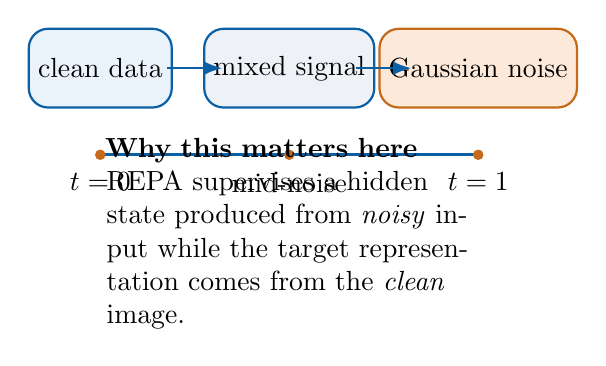
\begin{tikzpicture}[>=Latex,thick]
      \draw[line width=1pt,color=accent] (0,0) -- (4.8,0);
      \foreach \x/\label in {0/{\(t=0\)},2.4/{mid-noise},4.8/{\(t=1\)}} {
        \fill[color=signal] (\x,0) circle (1.9pt);
        \node[anchor=north] at (\x,-0.1) {\label};
      }
      \node[draw=accent,fill=accentlight,rounded corners=7pt,minimum width=1.65cm,minimum height=1.0cm] at (0,1.1) {clean data};
      \node[draw=accent,fill=softgray,rounded corners=7pt,minimum width=1.75cm,minimum height=1.0cm] at (2.4,1.1) {mixed signal};
      \node[draw=signal,fill=signalsoft,rounded corners=7pt,minimum width=1.65cm,minimum height=1.0cm] at (4.8,1.1) {Gaussian noise};
      \draw[->,color=accent] (0.85,1.1) -- (1.55,1.1);
      \draw[->,color=accent] (3.25,1.1) -- (3.95,1.1);
      \node[anchor=west,text width=4.85cm,align=left] at (-0.05,-1.0) {
        \textbf{Why this matters here}\\
        REPA supervises a hidden state produced from \emph{noisy} input while the target representation comes from the \emph{clean} image.
      };
    \end{tikzpicture}
  \end{columns}
\end{frame}

\begin{frame}[t]
  \framesubtitle{Method Setup}
  \frametitle{Training objective recap}
  \begin{columns}[T,totalwidth=\textwidth]
    \column{0.51\textwidth}
    \textbf{Velocity objective}
    \begin{align*}
      v(x,t) &= \dot{\alpha}_t \mathbb{E}[x^\ast \mid x_t=x] + \dot{\sigma}_t \mathbb{E}[\epsilon \mid x_t=x] \\
      \mathcal{L}_{\text{velocity}}(\theta) &= \mathbb{E}_{x^\ast,\epsilon,t}
      \left\|v_\theta(x_t,t) - \dot{\alpha}_t x^\ast - \dot{\sigma}_t \epsilon \right\|_2^2
    \end{align*}
    \vspace{0.1cm}
    \textbf{Reverse SDE}
    \begin{align*}
      dx_t = v(x_t,t)\,dt - \tfrac{1}{2}w_t s(x_t,t)\,dt + w_t\,d\bar{w}_t
    \end{align*}
  \column{0.47\textwidth}
    \textbf{Score from velocity}
    \begin{align*}
      s(x,t)=\sigma_t^{-1}\cdot
      \frac{\alpha_t v(x,t)-\dot{\alpha}_t x}
           {\dot{\alpha}_t \sigma_t - \alpha_t \dot{\sigma}_t}
    \end{align*}
    \vspace{0.16cm}
    \callout{\textbf{Interpretation.} The base denoising loss teaches the network to invert the corruption process.
    REPA adds a second pressure: hidden states should also look like clean, semantically structured visual features.}
    \vspace{0.16cm}
    {\small The paper applies this idea to both SiT-style velocity prediction and DiT-style DDPM objectives.}
  \end{columns}
\end{frame}

\begin{frame}[t]
  \framesubtitle{REPA}
  \frametitle{Intuition: noisy hidden states should predict clean semantics}
  \begin{columns}[T,totalwidth=\textwidth]
    \column{0.43\textwidth}
    \begin{itemize}
      \item A pretrained visual encoder sees the clean image \(x^\ast\) and produces target features \(y^\ast\).
      \item The diffusion transformer sees the noisy latent \(z_t\) and produces hidden state \(h_t\).
      \item A small projector maps \(h_t\) into the target feature space, and REPA aligns them patch by patch.
    \end{itemize}
    \vspace{0.14cm}
    \callout{\textbf{Why this is elegant.} We do not redesign sampling or the backbone. We only add a simple regularizer that distills external semantics into the denoising model.}
  \column{0.55\textwidth}
    \FigThree[width=\linewidth]
  \end{columns}
\end{frame}

\begin{frame}[t]
  \framesubtitle{REPA}
  \frametitle{Formal objective}
  \begin{columns}[T,totalwidth=\textwidth]
    \column{0.58\textwidth}
    \begin{align*}
      y^\ast &= f(x^\ast) \in \mathbb{R}^{N \times D} \\
      h_t &= f_\theta(z_t) \\
      \mathcal{L}_{\text{REPA}}(\theta,\phi) &=
      - \mathbb{E}_{x^\ast,\epsilon,t}
      \left[\frac{1}{N}\sum_{n=1}^N
      \mathrm{sim}\!\left(y_n^\ast, h_\phi(h_t)_n\right)\right]
    \end{align*}
    \begin{align*}
      \mathcal{L} = \mathcal{L}_{\text{velocity}} + \lambda \mathcal{L}_{\text{REPA}}
    \end{align*}
    \vspace{0.12cm}
    \begin{itemize}
      \item \(f\): frozen pretrained encoder, usually DINOv2
      \item \(h_\phi\): small trainable projection head
      \item \(\mathrm{sim}\): NT-Xent or cosine similarity
      \item \(\lambda\): tradeoff between denoising and alignment
    \end{itemize}
  \column{0.38\textwidth}
    \begin{beamercolorbox}[wd=\linewidth,rounded=true,sep=0.20cm]{block body}
      \textbf{Important design choice}\\
      The target comes from the \emph{clean image}, not from a noisy augmentation.
      So the model learns to recover semantic structure that is invariant to the diffusion corruption.
    \end{beamercolorbox}
    \vspace{0.18cm}
    \begin{beamercolorbox}[wd=\linewidth,rounded=true,sep=0.20cm]{block body}
      \textbf{Operationally}\\
      REPA is just an auxiliary loss. It slots into existing DiT / SiT training code with minimal structural change.
    \end{beamercolorbox}
  \end{columns}
\end{frame}

\begin{frame}[t]
  \framesubtitle{REPA}
  \frametitle{Architecture: where REPA is attached}
  \begin{columns}[T,totalwidth=\textwidth]
    \column{0.46\textwidth}
    \FigNine[width=\linewidth]
  \column{0.50\textwidth}
    \begin{itemize}
      \item Backbone stays identical to DiT / SiT: patchify latent image, run transformer blocks, predict denoising target.
      \item REPA reads an intermediate hidden state, typically from an early block.
      \item A lightweight 3-layer MLP projector is used only during training.
      \item AdaLN-zero conditioning and the standard denoising head remain untouched.
    \end{itemize}
    \vspace{0.15cm}
    \callout{\textbf{Practical takeaway.} REPA is not a new generator architecture. It is a training-time regularization layer on top of the existing architecture.}
  \end{columns}
\end{frame}

\begin{frame}[t]
  \framesubtitle{REPA}
  \frametitle{Why early-layer alignment is enough}
  \begin{columns}[T,totalwidth=\textwidth]
    \column{0.49\textwidth}
    \begin{tabular}{L{2.2cm}C{1.1cm}C{1.2cm}L{2.4cm}}
      \toprule
      Setting & Depth & FID \metricdown & Reading \\
      \midrule
      Vanilla SiT-L/2 & -- & 18.8 & no semantic guidance \\
      REPA + DINOv2-L & 6 & 10.3 & strong early gains \\
      REPA + DINOv2-L & 8 & 10.0 & best overall tradeoff \\
      REPA + DINOv2-L & 12 & 11.2 & later alignment starts to hurt \\
      REPA + DINOv2-L & 16 & 12.1 & less room for detail refinement \\
      \bottomrule
    \end{tabular}
  \column{0.47\textwidth}
    \begin{enumerate}
      \item Early blocks learn a semantic scaffold.
      \item Middle and late blocks no longer need to rediscover object-level structure.
      \item Remaining capacity can focus on high-frequency, generative detail.
    \end{enumerate}
    \vspace{0.18cm}
    \callout{\textbf{Interpretation from the paper.} REPA should shape the representation space early, then step out of the way so the model can finish the denoising task.}
  \end{columns}
\end{frame}

\begin{frame}[t]
  \framesubtitle{Experiments}
  \frametitle{What Table 2 says: the components that matter}
  \begin{columns}[T,totalwidth=\textwidth]
    \column{0.54\textwidth}
    \begin{tabular}{L{3.2cm}C{1.1cm}C{1.2cm}C{1.1cm}}
      \toprule
      Setting (SiT-L/2, 400K) & FID \metricdown & IS \metricup & Acc \metricup \\
      \midrule
      Vanilla & 18.8 & 72.0 & -- \\
      + MAE-L & 12.5 & 90.7 & 57.3 \\
      + CLIP-L & 11.0 & 100.4 & 67.2 \\
      + SigLIP-L & 10.2 & 107.0 & 68.8 \\
      + DINOv2-L & 10.0 & 106.6 & 68.1 \\
      + DINOv2-B & 9.7 & 107.5 & 65.7 \\
      + cosine similarity & 9.9 & 111.9 & 68.2 \\
      \bottomrule
    \end{tabular}
  \column{0.42\textwidth}
    \begin{itemize}
      \item Stronger target encoders improve both semantics and generation.
      \item Very large target encoders are \emph{not} mandatory; DINOv2-B already works well.
      \item Simple cosine similarity is competitive with contrastive objectives.
      \item REPA is robust: multiple design choices beat the vanilla baseline by a wide margin.
    \end{itemize}
  \end{columns}
\end{frame}

\begin{frame}[t]
  \framesubtitle{Experiments}
  \frametitle{Scalability: stronger targets and larger DiTs help more}
  \FigFive[width=\linewidth]
  \vspace{0.05cm}
  \begin{columns}[T,totalwidth=\textwidth]
    \column{0.32\textwidth}
    {\small \textbf{Target quality}\\
    Better pretrained encoders push both linear-probe accuracy and FID in the right direction.
    }
    \column{0.32\textwidth}
    {\small \textbf{Model size}\\
    Larger SiT models benefit more from REPA, so the relative speedup grows with scale.
    }
    \column{0.32\textwidth}
    {\small \textbf{Joint frontier}\\
    REPA improves the discrimination-generation frontier rather than trading one for the other.
    }
  \end{columns}
\end{frame}

\begin{frame}[t]
  \framesubtitle{Experiments}
  \frametitle{Convergence and efficiency}
  \begin{columns}[T,totalwidth=\textwidth]
    \column{0.48\textwidth}
    \FigEleven[width=\linewidth]
  \column{0.48\textwidth}
    \begin{tabular}{L{2.3cm}C{1.2cm}C{1.1cm}}
      \toprule
      Model & Iter. & FID \metricdown \\
      \midrule
      SiT-XL/2 & 7M & 8.3 \\
      REPA & 400K & 7.9 \\
      REPA & 1M & 6.4 \\
      REPA & 4M & 5.9 \\
      \midrule
      DiT-XL/2 & 7M & 9.6 \\
      REPA & 850K & 9.6 \\
      \bottomrule
    \end{tabular}
    \vspace{0.14cm}
    \callout{\textbf{Key message.} REPA is not only a better endpoint. It changes the optimization trajectory:
    the model gets into a good semantic regime much earlier.}
    \vspace{0.12cm}
    {\scriptsize The paper highlights a \(>17.5\times\) speedup for matching strong SiT performance without CFG.}
  \end{columns}
\end{frame}

\begin{frame}[t]
  \framesubtitle{Experiments}
  \frametitle{System-level comparison on ImageNet 256x256}
  \begin{columns}[T,totalwidth=\textwidth]
    \column{0.58\textwidth}
    \begin{tabular}{L{3.1cm}C{1.1cm}C{1.2cm}C{1.0cm}}
      \toprule
      Method & Epochs & FID \metricdown & Rec. \metricup \\
      \midrule
      U-ViT-H/2 & 240 & 2.29 & 0.57 \\
      DiffiT* & -- & 1.73 & 0.62 \\
      MDTv2-XL/2* & 1080 & 1.58 & 0.65 \\
      DiT-XL/2 & 1400 & 2.27 & 0.57 \\
      SiT-XL/2 & 1400 & 2.06 & 0.59 \\
      REPA (800 ep) & 800 & 1.80 & 0.61 \\
      REPA + guidance interval* & 800 & 1.42 & 0.64 \\
      \bottomrule
    \end{tabular}
  \column{0.38\textwidth}
    \begin{itemize}
      \item REPA beats vanilla SiT with fewer epochs.
      \item With CFG and guidance interval, it reaches the paper's best reported FID \(=1.42\).
      \item The gain is competitive against strong transformer and hybrid baselines.
    \end{itemize}
    \vspace{0.16cm}
    {\scriptsize * Rows marked with an asterisk use additional CFG scheduling / guidance interval from the cited setup.}
  \end{columns}
\end{frame}

\begin{frame}[t]
  \framesubtitle{Experiments}
  \frametitle{Qualitative improvement appears early in training}
  \FigFour[width=\linewidth]
  \vspace{0.06cm}
  \begin{columns}[T,totalwidth=\textwidth]
    \column{0.32\textwidth}
    {\small \textbf{Controlled comparison}\\
    Same noise, same sampler, same sampling steps, no CFG.
    }
    \column{0.32\textwidth}
    {\small \textbf{Visual pattern}\\
    REPA sharpens object identity and compositional structure earlier.
    }
    \column{0.32\textwidth}
    {\small \textbf{Interpretation}\\
    Better internal semantics translate into visibly better generations during the early training phase.
    }
  \end{columns}
\end{frame}

\begin{frame}[t]
  \framesubtitle{Interpretation}
  \frametitle{Why REPA helps both speed and final FID}
  \begin{center}
  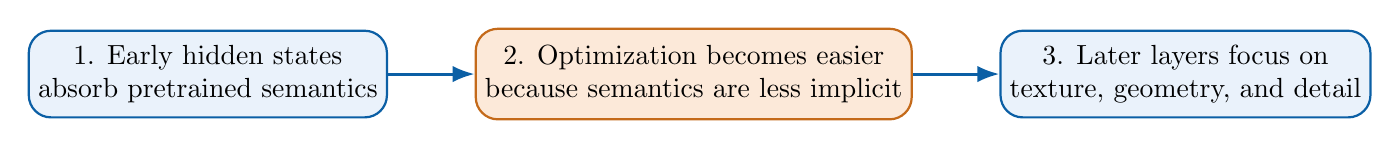
\begin{tikzpicture}[>=Latex,thick,node distance=1.15cm]
    \tikzstyle{ibox}=[draw=accent,fill=accentlight,rounded corners=8pt,minimum width=4.0cm,minimum height=1.1cm,align=center]
    \tikzstyle{gbox}=[draw=signal,fill=signalsoft,rounded corners=8pt,minimum width=4.2cm,minimum height=1.15cm,align=center]
    \node[ibox] (a) {1. Early hidden states\\ absorb pretrained semantics};
    \node[gbox,right=1.1cm of a] (b) {2. Optimization becomes easier\\ because semantics are less implicit};
    \node[ibox,right=1.1cm of b] (c) {3. Later layers focus on\\ texture, geometry, and detail};
    \draw[->,color=accent,line width=1.1pt] (a) -- (b);
    \draw[->,color=accent,line width=1.1pt] (b) -- (c);
  \end{tikzpicture}
  \end{center}
  \vspace{0.22cm}
  \begin{columns}[T,totalwidth=\textwidth]
    \column{0.48\textwidth}
    \callout{\textbf{Optimization story.} REPA supplies a clean semantic target that the denoising loss alone would need many more updates to discover.}
    \column{0.48\textwidth}
    \callout{\textbf{Quality story.} Once semantics are stabilized, the model can allocate more effective capacity to the truly generative part of the task.}
  \end{columns}
  \vspace{0.16cm}
  {\small This interpretation is empirical rather than theoretically proved, but it is consistent with the paper's ablations.}
\end{frame}

\begin{frame}[t]
  \framesubtitle{Discussion}
  \frametitle{Limitations and future directions}
  \begin{columns}[T,totalwidth=\textwidth]
    \column{0.52\textwidth}
    \begin{itemize}
      \item \textbf{Alignment depth} is chosen empirically; the paper does not fully explain why early layers are best.
      \item Most results are on \textbf{latent image diffusion}; video, pixel-space diffusion, and other modalities remain open.
      \item The work is mostly \textbf{empirical}; there is no strong theory for why this alignment objective works so well.
      \item The paper leaves \textbf{time-varying REPA weights} and richer schedules for future study.
    \end{itemize}
  \column{0.44\textwidth}
    \begin{beamercolorbox}[wd=\linewidth,rounded=true,sep=0.22cm]{block body}
      \textbf{Directions that look promising}
      \begin{itemize}
        \item larger-scale text-to-image training
        \item more principled alignment schedules
        \item theory linking denoising and representation learning
        \item broader encoder choices beyond current SSL vision models
      \end{itemize}
    \end{beamercolorbox}
  \end{columns}
\end{frame}

\begin{frame}[t]
  \framesubtitle{Takeaways}
  \frametitle{What to remember}
  \begin{columns}[T,totalwidth=\textwidth]
    \column{0.58\textwidth}
    \begin{enumerate}
      \item Diffusion transformers already learn useful features, but the features are not aligned enough with strong semantic representations.
      \item REPA converts that weakness into a simple auxiliary objective: align noisy hidden states to clean pretrained features.
      \item The result is one of the clearest cases where better representation learning directly improves generative training efficiency.
    \end{enumerate}
    \vspace{0.18cm}
    \callout{\textbf{Bottom line.} REPA is simple, modular, and high-leverage: it changes neither the sampler nor the backbone, yet materially changes the training dynamics.}
  \column{0.38\textwidth}
    \begin{beamercolorbox}[wd=\linewidth,rounded=true,sep=0.24cm]{block body}
      \textbf{Q\&A backup available}
      \begin{itemize}
        \item derivations
        \item metrics
        \item extra ablations
        \item 512x512 and T2I extensions
      \end{itemize}
    \end{beamercolorbox}
    \vspace{0.28cm}
    {\small Citation: S. Yu et al., ``Representation Alignment for Generation,'' ICLR 2025.}
  \end{columns}
\end{frame}


\appendix
\begin{frame}[t]
  \framesubtitle{Appendix}
  \frametitle{Backup roadmap}
  \begin{columns}[T,totalwidth=\textwidth]
    \column{0.48\textwidth}
    \begin{itemize}
      \item DDPM vs stochastic interpolants
      \item velocity / score relations
      \item CKNNA and linear probing
      \item DiT/SiT block details
      \item DiT analysis and more ablations
    \end{itemize}
  \column{0.48\textwidth}
    \begin{itemize}
      \item hyperparameters and compute
      \item detailed quantitative tables
      \item 512x512 extension
      \item text-to-image extension
      \item feature maps and extra qualitative samples
    \end{itemize}
  \end{columns}
\end{frame}

\begin{frame}[t]
  \framesubtitle{Appendix}
  \frametitle{DDPM vs stochastic interpolants}
  \begin{columns}[T,totalwidth=\textwidth]
    \column{0.48\textwidth}
    \textbf{DDPM view}
    \begin{itemize}
      \item discrete-time forward corruption with \(\beta_t\)
      \item learn reverse transitions \(p(x_{t-1}\mid x_t)\)
      \item common objective predicts noise \(\epsilon\)
    \end{itemize}
    \begin{align*}
      \mathcal{L}_{\text{simple}}
      = \mathbb{E}_{x^\ast,\epsilon,t}\left\|\epsilon-\epsilon_\theta(x_t,t)\right\|_2^2
    \end{align*}
  \column{0.48\textwidth}
    \textbf{Stochastic interpolant view}
    \begin{itemize}
      \item continuous path between data and Gaussian noise
      \item learn velocity or score over continuous time
      \item cleaner interface for flow-matching style models such as SiT
    \end{itemize}
    \begin{align*}
      x_t = \alpha_t x^\ast + \sigma_t \epsilon,\qquad
      \dot{x}_t = v(x_t,t)
    \end{align*}
    \vspace{0.12cm}
    {\small REPA is compatible with both views because it attaches to hidden representations rather than a specific sampler.}
  \end{columns}
\end{frame}

\begin{frame}[t]
  \framesubtitle{Appendix}
  \frametitle{Velocity and score relations}
  \begin{align*}
    v(x,t)
    &= \dot{\alpha}_t \mathbb{E}[x^\ast \mid x_t=x] + \dot{\sigma}_t \mathbb{E}[\epsilon \mid x_t=x] \\
    \mathcal{L}_{\text{velocity}}(\theta)
    &= \mathbb{E}_{x^\ast,\epsilon,t}
    \left\|v_\theta(x_t,t)-\dot{\alpha}_t x^\ast-\dot{\sigma}_t \epsilon\right\|_2^2
  \end{align*}
  \begin{align*}
    s(x,t) &= -\sigma_t^{-1}\mathbb{E}[\epsilon\mid x_t=x] \\
    s(x,t) &= \sigma_t^{-1}\cdot
    \frac{\alpha_t v(x,t)-\dot{\alpha}_t x}
         {\dot{\alpha}_t \sigma_t - \alpha_t \dot{\sigma}_t}
  \end{align*}
  \vspace{0.1cm}
  \callout{\textbf{Why these equations matter for REPA.} The paper keeps the denoising math intact.
  REPA only adds feature supervision on top of the same hidden states used to solve these objectives.}
\end{frame}

\begin{frame}[t]
  \framesubtitle{Appendix}
  \frametitle{What are CKNNA and linear probing measuring?}
  \begin{columns}[T,totalwidth=\textwidth]
    \column{0.52\textwidth}
    \textbf{Linear probing}
    \begin{itemize}
      \item Freeze the representation.
      \item Train a linear classifier on ImageNet labels.
      \item Higher accuracy implies stronger semantic separability.
    \end{itemize}
    \vspace{0.16cm}
    \textbf{CKNNA}
    \begin{itemize}
      \item A relaxed alignment metric related to CKA.
      \item Focuses on mutual nearest neighbors rather than all pairwise relationships.
      \item More forgiving when comparing representations from different model families.
    \end{itemize}
  \column{0.44\textwidth}
    \begin{align*}
      \mathrm{CKA}(K,L)
      =
      \frac{\mathrm{HSIC}(K,L)}
      {\sqrt{\mathrm{HSIC}(K,K)\mathrm{HSIC}(L,L)}}
    \end{align*}
    \begin{beamercolorbox}[wd=\linewidth,rounded=true,sep=0.18cm]{block body}
      \textbf{How the paper uses them}
      \begin{itemize}
        \item probing: semantic gap
        \item CKNNA: representational alignment
      \end{itemize}
    \end{beamercolorbox}
  \end{columns}
\end{frame}

\begin{frame}[t]
  \framesubtitle{Appendix}
  \frametitle{DiT / SiT block details}
  \begin{columns}[T,totalwidth=\textwidth]
    \column{0.42\textwidth}
    \FigNine[width=\linewidth]
  \column{0.54\textwidth}
    \begin{itemize}
      \item Patchified latent tokens go through repeated attention + MLP blocks.
      \item AdaLN-zero style modulation injects timestep and condition information.
      \item REPA taps one intermediate hidden state and sends it to a separate projection MLP.
      \item The projection head is a training-time adapter into the external encoder feature space.
    \end{itemize}
  \end{columns}
\end{frame}

\begin{frame}[t]
  \framesubtitle{Appendix}
  \frametitle{The same behavior also appears in DiT}
  \begin{columns}[T,totalwidth=\textwidth]
    \column{0.47\textwidth}
    \FigTen[width=\linewidth]
  \column{0.49\textwidth}
    \begin{itemize}
      \item DiT hidden states also show a semantic gap relative to DINOv2.
      \item Alignment is present but weak, just like in SiT.
      \item So the paper's argument is not a SiT-only artifact; it generalizes across denoising transformer families.
    \end{itemize}
  \end{columns}
\end{frame}

\begin{frame}[t]
  \framesubtitle{Appendix}
  \frametitle{More ablations: timesteps, target encoders, and \(\lambda\)}
  \begin{columns}[T,totalwidth=\textwidth]
    \column{0.58\textwidth}
    \papercrop[width=\linewidth]{10}{70bp 320bp 60bp 88bp}
  \column{0.38\textwidth}
    \begin{itemize}
      \item REPA improves the representation gap across multiple noise levels.
      \item Alignment gains are not specific to DINOv2; MAE and MoCov3 also show the trend.
      \item Performance is fairly robust once \(\lambda\) reaches about \(0.5\).
    \end{itemize}
    \vspace{0.14cm}
    \begin{tabular}{C{1.0cm}C{1.0cm}C{1.0cm}C{1.0cm}}
      \toprule
      \(\lambda\) & 0.25 & 0.5 & 1.0 \\
      \midrule
      FID & 8.6 & 7.9 & 7.8 \\
      \bottomrule
    \end{tabular}
  \end{columns}
\end{frame}

\begin{frame}[t]
  \framesubtitle{Appendix}
  \frametitle{Hyperparameters and compute details}
  \begin{columns}[T,totalwidth=\textwidth]
    \column{0.60\textwidth}
    \begin{tabular}{L{2.8cm}L{3.8cm}}
      \toprule
      Category & Setup used in the paper \\
      \midrule
      Backbone & same DiT / SiT architecture as original papers \\
      Input & ImageNet 256x256, VAE latents of size \(32\times32\times4\) \\
      Optimizer & AdamW, learning rate \(1\times 10^{-4}\), no weight decay \\
      Batch size & 256 \\
      Sampler & Euler-Maruyama, \(w_t=\sigma_t\), NFE \(=250\) \\
      Projection head & 3-layer MLP with SiLU \\
      Training hardware & 8x H100 80GB, about 5.4 step/s \\
      \bottomrule
    \end{tabular}
  \column{0.34\textwidth}
    \callout{\textbf{Engineering note.} The paper mentions that training can be sped up further by precomputing pretrained-encoder features.}
  \end{columns}
\end{frame}

\begin{frame}[t]
  \framesubtitle{Appendix}
  \frametitle{Detailed quantitative results}
  \begin{columns}[T,totalwidth=\textwidth]
    \column{0.48\textwidth}
    \begin{tabular}{L{2.1cm}C{1.0cm}C{0.9cm}C{1.0cm}}
      \toprule
      Model & Iter. & FID & Acc. \\
      \midrule
      SiT-B/2 + REPA & 400K & 24.4 & 61.2 \\
      SiT-L/2 + REPA & 400K & 10.0 & 69.4 \\
      SiT-XL/2 + REPA & 400K & 7.9 & 70.3 \\
      SiT-XL/2 + REPA & 4M & 5.9 & 74.6 \\
      \bottomrule
    \end{tabular}
    \vspace{0.16cm}
    {\small Larger models gain more from REPA, and the advantage keeps growing with longer training.}
    \column{0.48\textwidth}
    \begin{tabular}{L{2.5cm}C{0.8cm}C{0.9cm}}
      \toprule
      Setting & \(w\) & FID \\
      \midrule
      Vanilla SiT-XL/2 & 1.50 & 2.06 \\
      REPA & 1.30 & 1.80 \\
      REPA + interval [0,0.75] & 2.00 & 1.78 \\
      REPA + interval [0,0.70] & 1.80 & 1.42 \\
      \bottomrule
    \end{tabular}
    \vspace{0.16cm}
    {\small Guidance interval plus REPA produces the best reported ImageNet 256x256 result in the paper.}
  \end{columns}
\end{frame}

\begin{frame}[t]
  \framesubtitle{Appendix}
  \frametitle{Extension to ImageNet 512x512}
  \begin{columns}[T,totalwidth=\textwidth]
    \column{0.60\textwidth}
    \AppFiveTwelve[width=\linewidth]
  \column{0.36\textwidth}
    \begin{itemize}
      \item Same setup idea, larger latent input.
      \item REPA already beats vanilla SiT-XL/2 with \(>3\times\) fewer iterations.
      \item Shows the method scales beyond the 256x256 headline experiment.
    \end{itemize}
  \end{columns}
\end{frame}

\begin{frame}[t]
  \framesubtitle{Appendix}
  \frametitle{Text-to-image extension}
  \begin{columns}[T,totalwidth=\textwidth]
    \column{0.64\textwidth}
    \AppTTwoI[width=\linewidth]
  \column{0.32\textwidth}
    \begin{itemize}
      \item The paper also applies REPA to MMDiT on MS-COCO.
      \item Reported FID improves from 6.05 to 4.73 in the ODE setup, and from 5.30 to 4.14 in the SDE setup.
      \item This suggests the alignment idea remains useful even when text conditioning is present.
    \end{itemize}
  \end{columns}
\end{frame}

\begin{frame}[t]
  \framesubtitle{Appendix}
  \frametitle{Feature maps and extra qualitative samples}
  \begin{columns}[T,totalwidth=\textwidth]
    \column{0.62\textwidth}
    \AppFeature[width=\linewidth]
  \column{0.34\textwidth}
    \AppQualTop[width=\linewidth]
    \vspace{0.14cm}

    \AppQualBottom[width=\linewidth]
  \end{columns}
\end{frame}


\end{document}
